\documentclass[11pt,letterpaper]{article}
\usepackage[utf8]{inputenc}
\usepackage[english]{babel}
\usepackage{graphicx}
\usepackage{amsfonts}
\usepackage{multicol}
\usepackage{flushend}
\usepackage{float}
\usepackage{fancyhdr}
\usepackage{colortbl}
\usepackage{amssymb}
\usepackage[margin=0.5 in]{geometry}
\usepackage{hyperref}
\usepackage{amsmath}
\usepackage{diagbox, eqparbox, hhline}
\usepackage{amssymb}

\renewcommand{\theequation}{\arabic{equation}}
\newcounter{neq}

\begin{document}
\setlength{\unitlength}{1cm}
\thispagestyle{empty}
\begin{picture}(18,4)
\put(0.5,0.2){
\includegraphics[scale=.35]{./img/unam1}}
\put(14.5,0){
\includegraphics[scale=.4]{./img/fciencias1}}
\end{picture}

\begin{center}
\textbf{{\LARGE Universidad Nacional Autónoma de México}}\\[0.2cm]
\textbf{{\LARGE Facultad de Ciencias\\Castro Mejia Jonatan Alejandro 314027687\\Leyva Castillo Luis Angel 314050577\\~\\Rosado Cabrera Diego 314293804}}\\[0.2cm]
\end{center}
\section{XSS}
\begin{center}
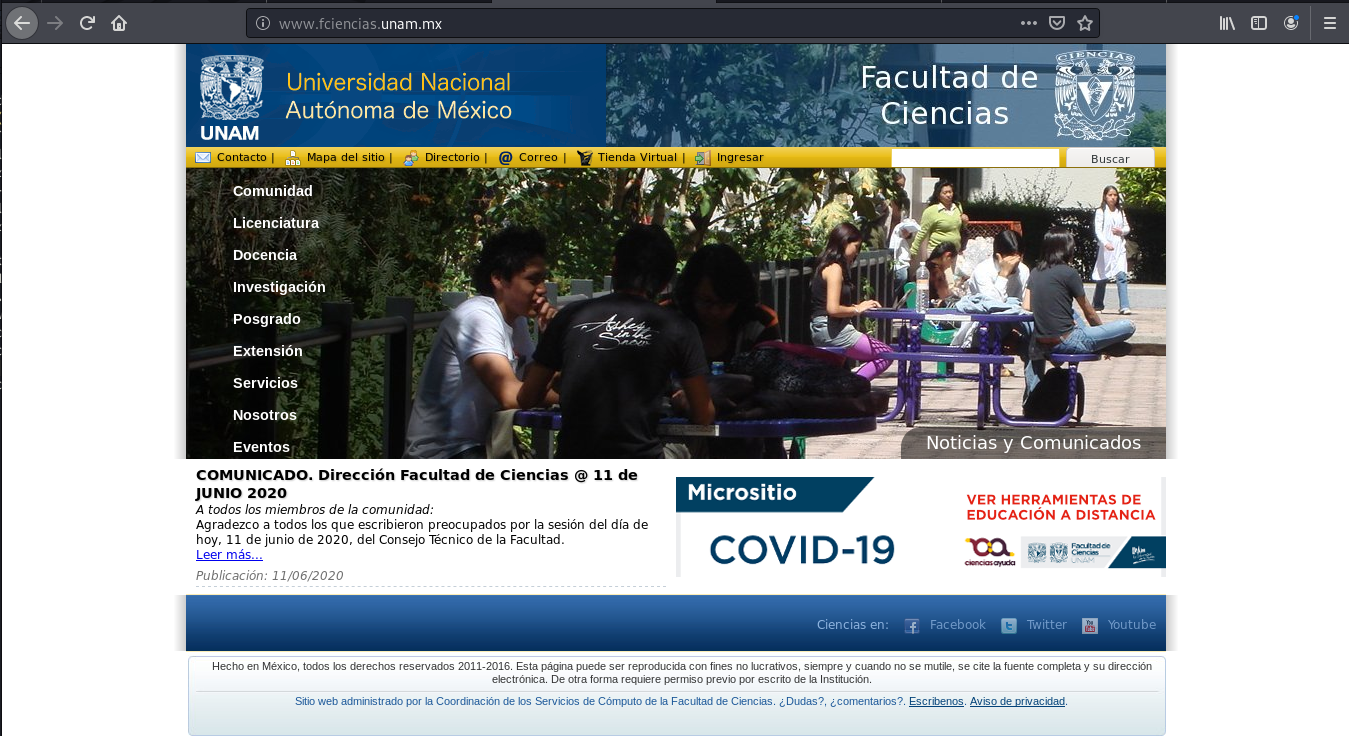
\includegraphics[scale=.4]{./Img/img0.png}
\end{center}~\\~\\~\\
\begin{center}
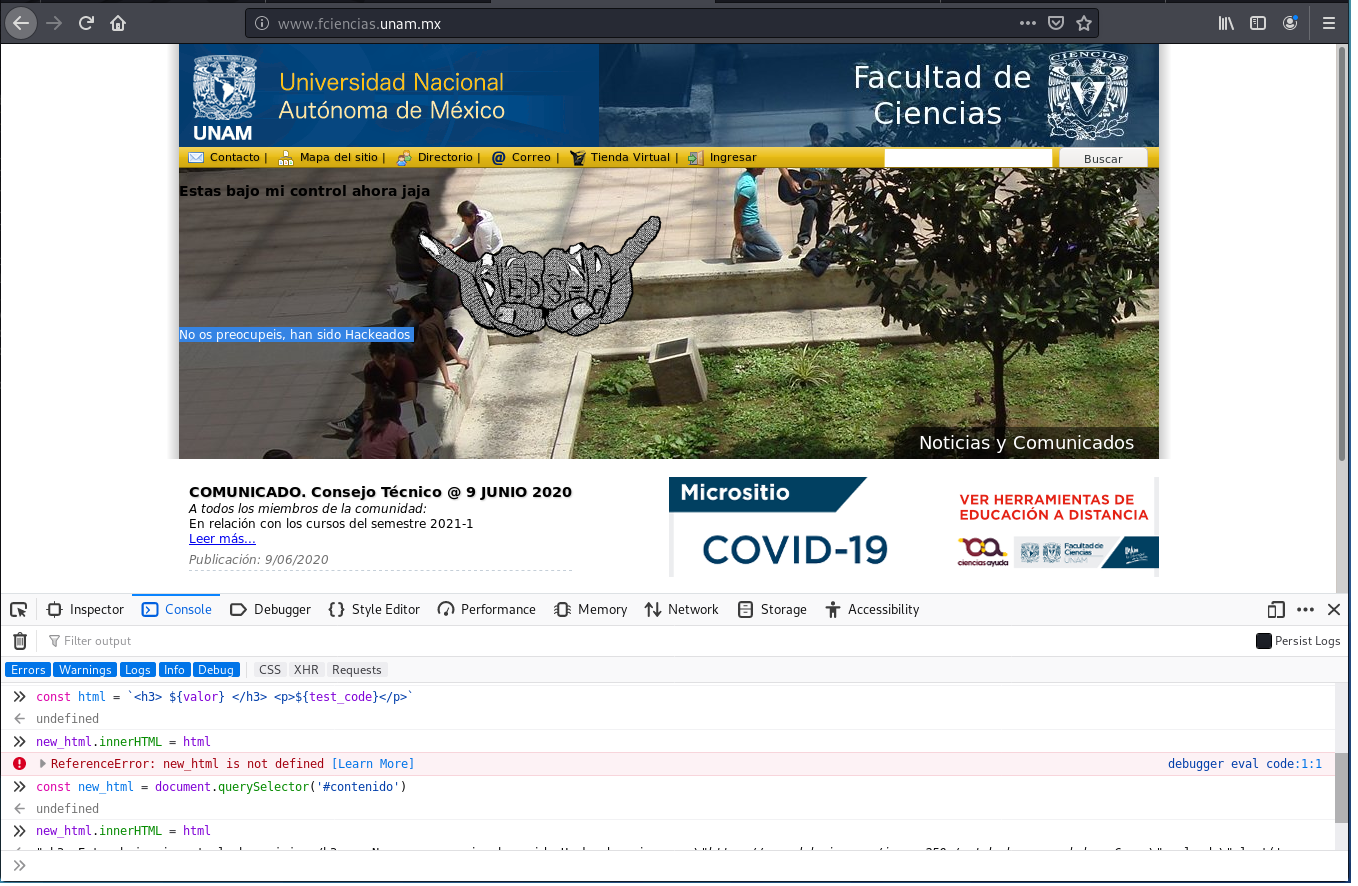
\includegraphics[scale=.4]{./Img/img1.png}
\end{center}~\\~\\~\\
\begin{center}
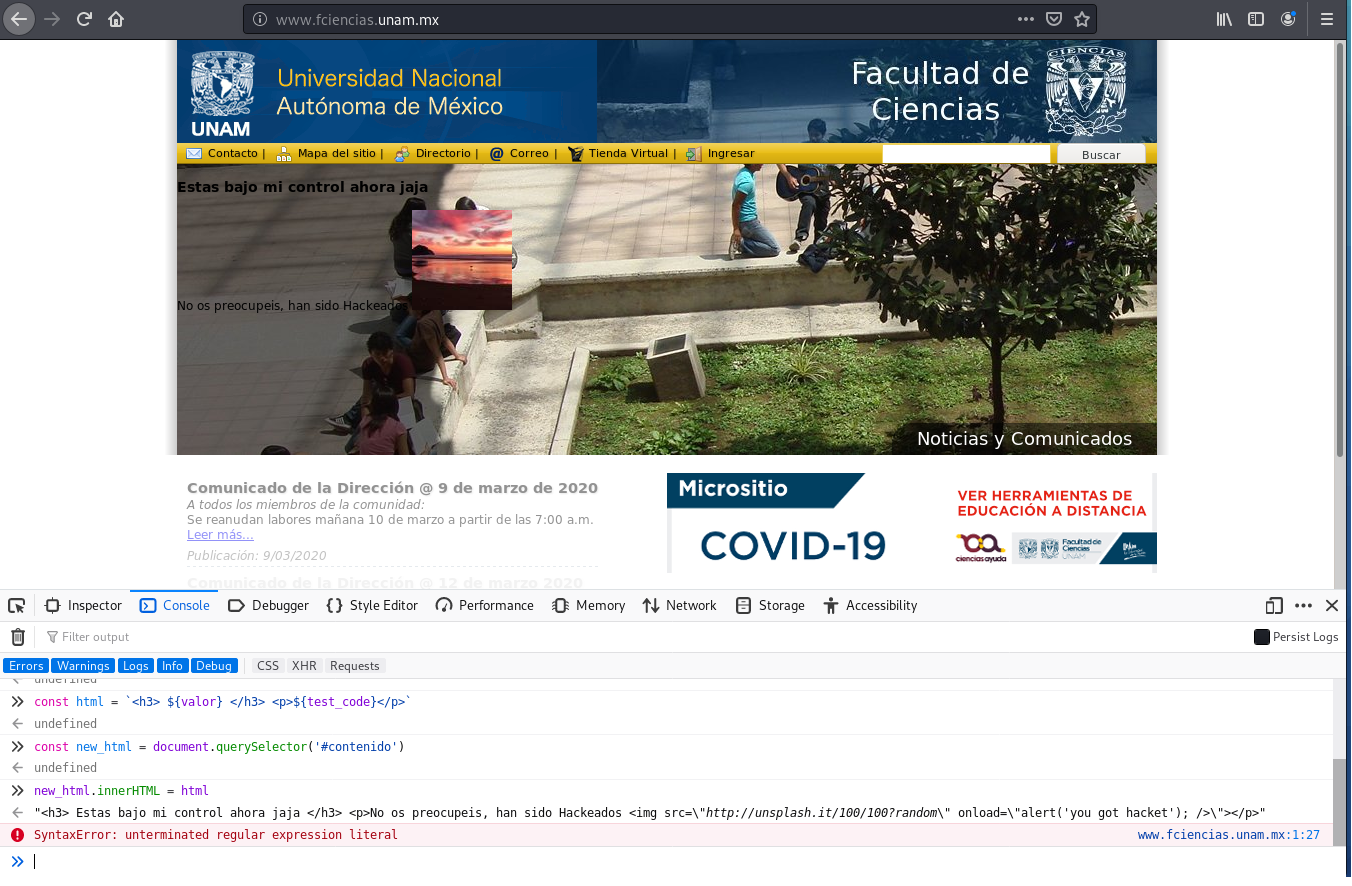
\includegraphics[scale=.4]{./Img/img2.png}
\end{center}~\\~\\~\\
\section{SQL Injection}
*Se adjunta el Script de los comandos utilizados.
%Para XSS, encontrar un sitio web que presente esta vulnerabilidad, e inyectar una imagen de un servicio remoto, así como mostrar que se puede ejecutar código JavaScript ajeno a la página web original. Incluir captura de pantalla del sitio web que muestre el antes y el después de la ejecución del código XSS.
%sPara SQLinjection, utilizar la herramienta sqlmap. Con base en la documentación de sqlmap y el análisis de los comandos vistos en clase, obtener el usuario y contraseña para el sitio:
Primero accedemos a la pagina como se muestra en la imagen, notamos que el url no posee algún id, por lo que procedemos a darle click al 1 (el cual nos da la categoría 1).\\
\begin{center}
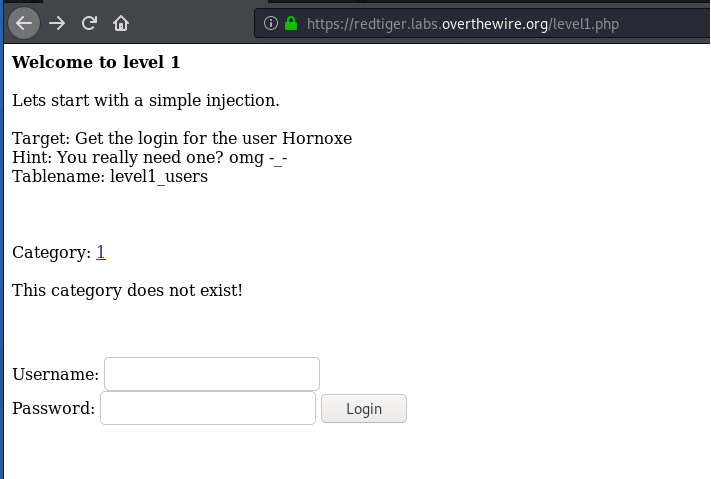
\includegraphics[scale=.6]{./Img/sqlmap0.png}
\end{center}~\\~\\~\\
Se observa que se actualiza el url mostrando la categoría 1, por lo que podemos proceder a ejecutar sqlmap para obtener la información que necesitamos.\\
\begin{center}
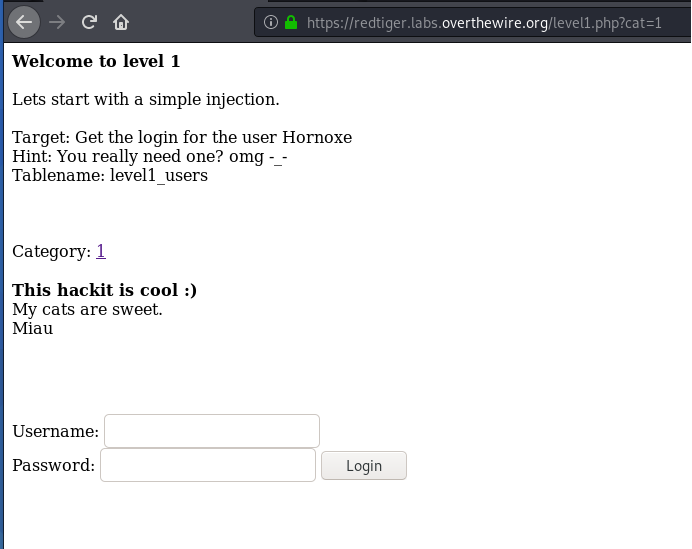
\includegraphics[scale=.6]{./Img/sqlmap1.png}
\end{center}~\\~\\~\\
Ejecutando el comando <comando1> se obtiene el nombre de la base de datos.\\
Parámetros usados: -u y --dbs
\begin{center}
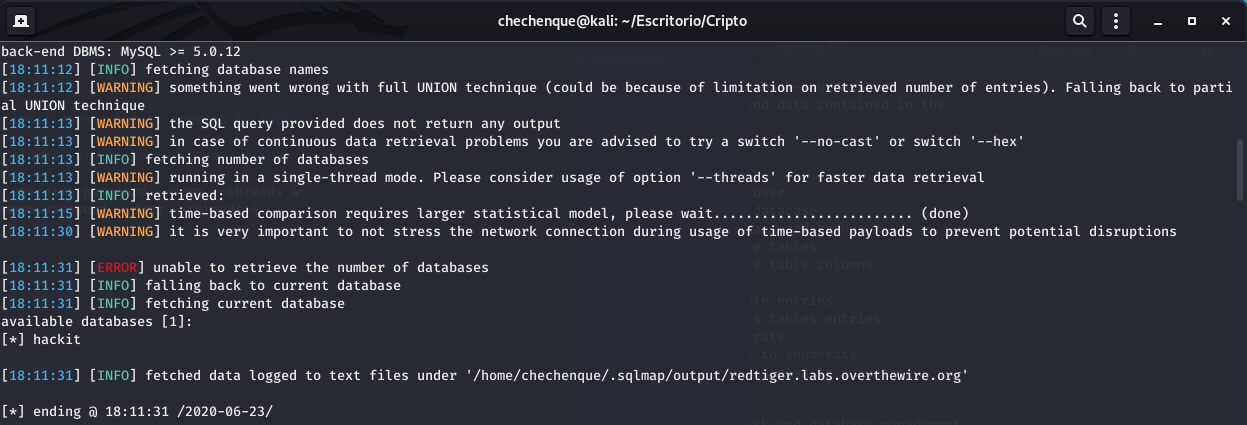
\includegraphics[scale=.5]{./Img/sqlmap2.png}
\end{center}~\\~\\~\\
Una vez obtenido el nombre de la base, tenemos que sacar el nombre de las tablas (aunque la pagina ya nos da el nombre de la tabla, lo hacemos por fines didácticos y por explicación de la herramienta), utilizando lel comando <comando2> se obtiene las tablas.\\
Parametros utilizados: -u, -D --tables\\
\begin{center}
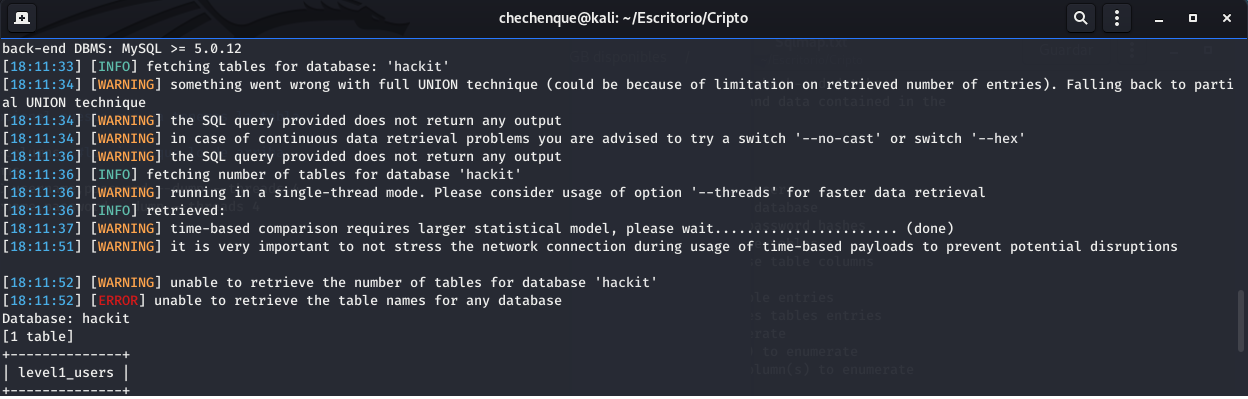
\includegraphics[scale=.5]{./Img/sqlmap3.png}
\end{center}~\\~\\~\\
\begin{center}
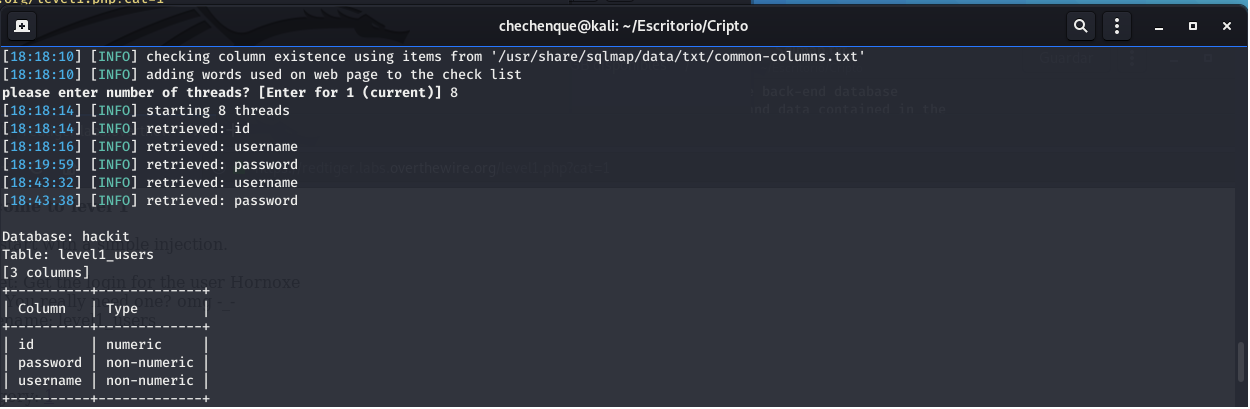
\includegraphics[scale=.5]{./Img/sqlmap4.png}
\end{center}~\\~\\~\\
\begin{center}
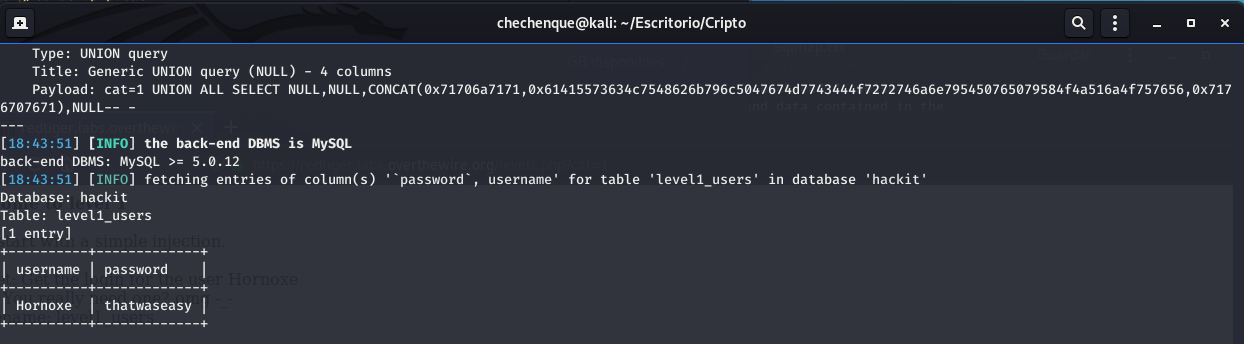
\includegraphics[scale=.5]{./Img/sqlmap5.png}
\end{center}~\\~\\~\\
\begin{center}
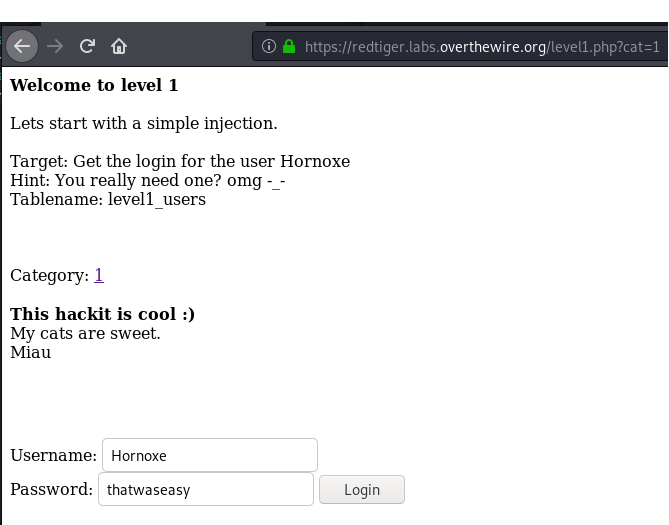
\includegraphics[scale=.6]{./Img/sqlmap6.png}
\end{center}~\\~\\~\\
\begin{center}
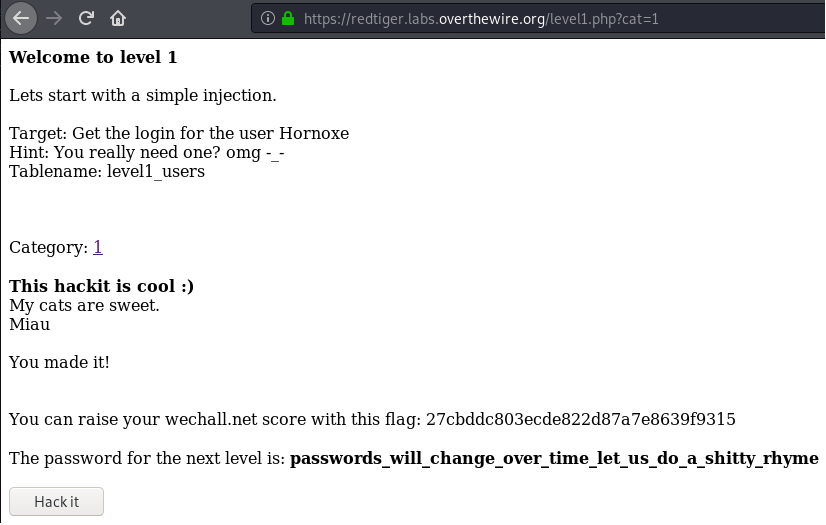
\includegraphics[scale=.6]{./Img/sqlmap7.png}
\end{center}~\\~\\~\\
\end{document}